
\noindent The building blocks of a quantum field theory are the observables, $n$-point Green's functions in the Heisenberg picture

\begin{equation}
G^{(n)}_{\alpha} (\textbf{x}_1, \dots, \textbf{x}_n) \equiv \bra{\Omega} \mathcal{T} [ \hat{\Phi}_{\alpha_1} (\textbf{x}_1) \dots \hat{\Phi}_{\alpha_n} (\textbf{x}_n) ] \ket{\Omega}
\end{equation}

\noindent Where $\ket{\Omega}$ is the full interacting vacuum state and $\alpha$ is a vector denoting all relevant quantum fields. \\
\noindent For example, in a theory of scalar bosons and fermions the field operators may be labeled as

\begin{align*}
\hat{\Phi}_0 (\textbf{x}) = \hat{\phi}(\textbf{x}) &\text{  for a scalar boson} \\
\hat{\Phi}_\alpha (\textbf{x}) = \hat{\psi}_\alpha (\textbf{x}) &\text{  for a Dirac spinor, }  \alpha = 1, 2, 3, 4
\end{align*}

\noindent We make predictions perturbatively by the general form of the Hamiltonian $\hat{H} = \hat{H}_{free} + \hat{H}_{int}$, where $\hat{H}_{free}$ just contains independent copies of the bosonic and fermionic fields, and $\hat{H}_{int}$ contains cross-terms. \\

\noindent For example, we may have the following free Hamiltonian combining the Klein-Gordon and Dirac fields.

\begin{align}
\hat{H}_{free} &= \hat{H}_{KG} + \hat{H}_{Dirac} \\
&= \left( \frac{1}{2} \int d^3 x \,\, \hat{\pi}^2 (x) + m^2 \hat{\phi}^2 (x) + (\nabla \hat{\phi} (x) )^2 \right) + \left( \int d^3 x \,\, \hat{\psi}^\dagger ( -i \gamma^0 \underline{\gamma} \cdot \underline{\nabla} + m \gamma^0 ) \hat{\psi} \right) .
\end{align}

\noindent And the interacting Hamiltonian with bosons interacting via the $\phi^4$ interaction and bosons and fermions interacting via the second term (Yukawa theory) containing the simplest Lorentz-invariant Dirac spinor quantity $\hat{\bar{\psi}} \hat{\psi}$ (Lorentz scalar from the Lagrangian density). Note that if $\phi^4$ is the only interaction, everything decouples.

\begin{equation}
\hat{H}_{int} = \int d^3 x \,\, \frac{\lambda}{4!} \hat{\phi}^4 (x) + g \hat{\phi} (x) \hat{\bar{\psi}} (x) \hat{\psi} (x)
\end{equation}

\noindent Recall that the equation used to solve for $G^{(n)}$ is

\begin{equation}
G^{(n)}_\alpha (\textbf{x}_1, \dots, \textbf{x}_n) = \frac{\bra{0} \mathcal{T} [\hat{\Phi}_{\alpha_1} (\textbf{x}_1) \dots \hat{\Phi}_{\alpha_n} (\textbf{x}_n) \mathcal{S} ] \ket{0}}{\bra{0} \mathcal{S} \ket{0}}
\end{equation}

\noindent Which uses the scattering matrix $\mathcal{S} = \lim_{t \rightarrow \infty} U(t, -t)$ (see Lecture 8), which can be expanded perturbatively via the Dyson series

\begin{equation}
U(t, -t) = \mathbb{I} - i \int^t_{-t} dt' \hat{H}_{int} (t') + (-i)^2 \int^t_{-t} dt' \int^{t'}_{-t'} dt'' \hat{H}_{int} (t') \hat{H}_{int} (t'') + \dots .
\end{equation}

\noindent After substituting the Dyson series for the scattering matrix, the correlation function is calculated order-by-order, which runs into infinities. We therefore introduced the cutoff for the interacting Hamiltonian up to some scale $\Lambda$

\begin{equation}
\hat{H}_{int} \rightarrow \hat{H}_{int} (\Lambda). 
\end{equation}

\noindent After all, terms in the series for $G^{(n)}$ are time-ordered products of the field operators in the interaction picture $\bra{0}  \mathcal{T} [\hat{\Phi} (z_1) \dots \hat{\Phi} (z_m) ] \ket{0}$ and integrals over $z_1, \dots, z_m$, where Wick's theorem is used to evaluate the time-ordered product. We now generalize Wick's theorem to fermionic (spinor) field operators.

\subsection*{Wick's Theorem for Fermions}

\noindent Define the time-ordering symbol for fermionic field operators with spinor labels $\alpha, \beta = 1, 2, 3, 4$, and note that the product of the two field operators is actually 16 operators in total.

\begin{equation}
\mathcal{T} [ \hat{\psi}_\alpha (\textbf{x}) \hat{\bar{\psi}}_\beta (\textbf{y}) ] =
	\begin{cases}
      		\hat{\psi}_\alpha (\textbf{x}) \hat{\bar{\psi}}_\beta (\textbf{y}) , & x^0 \ge y^0 \\
      		-\hat{\bar{\psi}}_\beta (\textbf{y})\hat{\psi}_\alpha (\textbf{x}) , & x^0 < y^0
    	\end{cases}
\end{equation}

\noindent Recall the Feynman propagator calculated from the time-ordered products contains 16 numbers in total. For two fermionic field operators we can define the time-ordering as

\begin{equation}
S_F^{\alpha \beta} = \int \frac{d^4 p}{(2 \pi)^4} \,\, \frac{i (\slashed{p} + m \cdot \mathbb{I})_{\alpha \beta} }{ p^2 - m^2 + i \epsilon} e^{-i \textbf{p} \cdot (\textbf{x} - \textbf{y})} \equiv \bra{0} \mathcal{T} [ \hat{\psi}_\alpha (\textbf{x}) \hat{\bar{\psi}}_\beta (\textbf{y}) ] \ket{0} \equiv \wick[offset=1.5em]{\c {\hat{\psi} (\textbf{x})} \c {\hat{\bar{\psi}} (\textbf{y})}}.
\end{equation}

\noindent Now we generalize $\mathcal{T}[]$ to many fermionic field operators

\begin{equation}
\mathcal{T} [ \hat{\psi} (\textbf{x}_1) \dots \hat{\psi} (\textbf{x}_n) ] = (-1)^{sgn(\pi)} \hat{\psi} (\textbf{x}_{\pi^{-1}(1)}) \dots \hat{\psi} (\textbf{x}_{\pi^{-1}(n)})
\end{equation}

\noindent Where $x^0_{\pi^{-1}(1)} > \dots > x^0_{\pi^{-1}(n)} $, for $\pi \in S_n$ the symmetric group. \\

\noindent To prove Wick's theorem and produce a workable form of the equation, the base case of Wick's theorem for fermions starts with two field operators, relating the time-ordered product to the normal-ordered product and the Wick contraction

\begin{equation}
\mathcal{T} [ \hat{\psi} (\textbf{x}) \hat{\bar{\psi}} (\textbf{y}) ] = \mathcal{N} [ \hat{\psi} (\textbf{x}) \hat{\bar{\psi}} (\textbf{y}) ] + \wick[offset=1.5em]{\c {\hat{\psi} (\textbf{x})} \c {\hat{\bar{\psi}} (\textbf{y})}}.
\end{equation}

\noindent Explicitly, the Wick contraction can be written in terms of the anticommutation brackets for positive and negative frequencies (antiparticles) and related to the Feynman propagator (\textbf{Exercise})

\begin{equation}
\wick[offset=1.5em]{\c {\hat{\psi} (\textbf{x})} \c {\hat{\bar{\psi}} (\textbf{y})}} = S_F (\textbf{x} - \textbf{y}) = 
	\begin{cases}
		\{ \hat{\psi}^+ (\textbf{x}), \hat{\bar{\psi}}^- (\textbf{y}) \} , \,\, x^0 \ge y^0 \\
		\{ \hat{\bar{\psi}}^+ (\textbf{y}) , \hat{\psi}^- (\textbf{x}) \}, \,\, x^0 < y^0.
	\end{cases}
\end{equation}

\noindent For ``non-mixed`` field operators, the Wick contraction is zero

\begin{equation}
\wick[offset=1.5em]{\c {\hat{\psi} (\textbf{x})} \c {\hat{\psi} (\textbf{y})}} = \wick[offset=1.5em]{\c {\hat{\bar{\psi} }(\textbf{x})} \c {\hat{\bar{\psi}} (\textbf{y})}} = 0.
\end{equation}

\noindent Now we extend the normal ordering principle to account for operator interchange, since each interchange of fermionic field operators introduces a minus sign to the product. For example,

\begin{equation}
\mathcal{N} [ \wick[offset=1.5em]{\c {\hat{\psi}_1} \hat{\psi}_2 \c {\hat{\bar{\psi}}_3} \hat{\bar{\psi}}_4 } ] = (-1) \wick[offset=1.5em]{\c {\hat{\psi}_1} \c {\hat{\bar{\psi}}_3} } \mathcal{N} [ \hat{\psi}_2 \hat{\bar{\psi}}_4 ] = (-1) S_F (\textbf{x}_1 - \textbf{x}_3) \mathcal{N} [ \hat{\psi}_2 \hat{\bar{\psi}}_4 ].
\end{equation}

\noindent WIth this, we extrapolate to the full Wick's theorem, which will be the same as the bosonic case except for minus signs introduced from moving contracted operators next to each other, for fermionic field operators that allows us to calculate time-ordered products of $n$ field operators in terms of the normal-ordered sum of all possible Wick contractions, and, in turn, in terms of Feynman propagators

\begin{equation}
\mathcal{T} [ \hat{\psi}_1 \hat{\bar{\psi}}_2 \dots ] = \mathcal{N} [ \hat{\psi}_1 \hat{\bar{\psi}}_2 \dots + \text{``all possible contractions''} ].
\end{equation}

\subsection*{Schematic of Perturbative QFT Calculation }

\noindent Begin with the observables and relate them to field operators in the interaction picture

\begin{equation}
G^{(n)}_\alpha (\textbf{x}_1, \dots, \textbf{x}_n) = \frac{\bra{0} \mathcal{T} [\hat{\Phi}_{\alpha_1} (\textbf{x}_1) \dots \hat{\Phi}_{\alpha_n} (\textbf{x}_n) \mathcal{S} ] \ket{0}}{\bra{0} \mathcal{S} \ket{0}}
\end{equation}

\noindent Apply the Dyson expansion to the scattering matrix, and then apply Wick's theorem

\begin{align}
G^{(n)}_\alpha (\textbf{x}_1, \dots, \textbf{x}_n) &= \mathbb{I} + \int dz \,\, \wick[offset=1.5em]{\c {\hat{\Phi}(z)} \c {\hat{\Phi}(z)}} + \int\int dz \,\, \wick[offset=1.5em]{\c {\hat{\Phi}(z)} \c {\hat{\Phi}(z)}} \wick[offset=1.5em]{\c {\hat{\Phi}(z)} \c {\hat{\Phi}(z)}} + \dots \\
&=
\end{align}

\begin{figure}[H]\centering 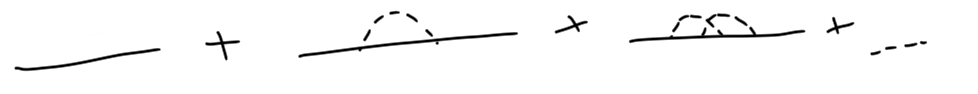
\includegraphics[scale=0.4]{lots.png}  \end{figure}

\noindent The end result if the sum of very many integrals of Wick contractions, and Feynman rules, dependent on the form of $\hat{H}_{int}$, are used to exploit patterns and cancellations in the terms. 

\subsection*{Example: Yukawa Theory}

\noindent Consider the Hamiltonian with interaction based on the fermion density $\hat{\bar{\psi}} \hat{\psi}$ and a single boson field $\hat{\phi}$, make the boson field sensitive to the density of the fermion field

\begin{equation}
\hat{H} =\hat{H}_{KG} + \hat{H}_{Dirac} + \int d^3 x \,\, g \, \hat{\bar{\psi}}(x) \hat{\psi}(x) \hat{\phi}(x).
\end{equation}

\noindent The Feynman rules in momentum space for this quantum field theory are, with dashed lines for bosons and solid lines for fermios

\begin{enumerate}
\item Propagators
	\subitem $\wick[offset=1.5em]{\c {\hat{\phi}(x)} \c {\hat{\phi}(y)}} = \frac{i}{p^2 - m_\phi^2 + i \epsilon} = $ \begin{figure}[H]\centering 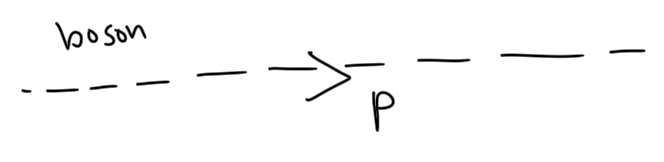
\includegraphics[scale=0.3]{bosonprop.png}  \end{figure}
	\subitem $\wick[offset=1.5em]{\c {\hat{\psi}(x)} \c {\hat{\bar{\psi}}(y)}} = \frac{i (\slashed{p} + m)}{p^2 - m^2 + i \epsilon} = $ \begin{figure}[H]\centering 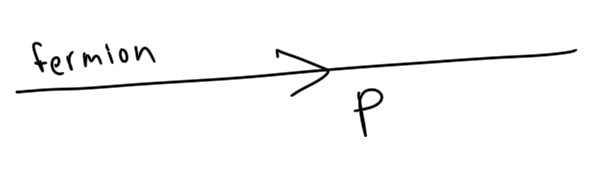
\includegraphics[scale=0.3]{fermionprop.png}  \end{figure}
\item Vertices
	\subitem $-ig = $ \begin{figure}[H]\centering 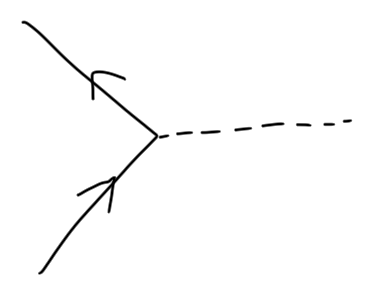
\includegraphics[scale=0.3]{vertex.png}  \end{figure}
\item External Legs
	\subitem $\wick[offset=1.5em]{\c {\hat{\phi}} \c {\ket{q}}} = 1 = $ \begin{figure}[H]\centering 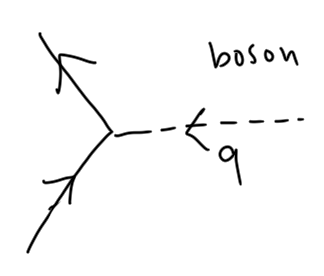
\includegraphics[scale=0.5]{bosonket.png}  \end{figure}
	\subitem $\wick[offset=1.5em]{\c {\bra{q}} \c {\hat{\phi}}} = 1 = $ \begin{figure}[H]\centering 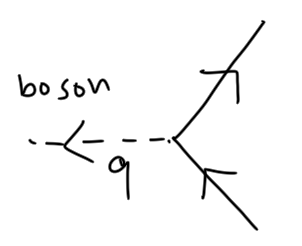
\includegraphics[scale=0.5]{bosonbra.png}  \end{figure}
	\subitem $\wick[offset=1.5em]{\c {\hat{\psi}} \c {\ket{p,s}}} = u^s (p) = $ \begin{figure}[H]\centering 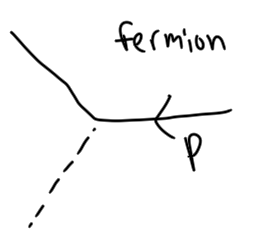
\includegraphics[scale=0.5]{fermionket.png}  \end{figure}
	\subitem $\wick[offset=1.5em]{\c {\bra{p,s}} \c {\hat{\bar{\psi}}}} = \bar{u}^s (p) = $ \begin{figure}[H]\centering 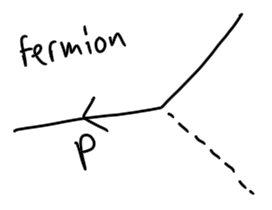
\includegraphics[scale=0.5]{fermionbra.png}  \end{figure}
	\subitem $\wick[offset=1.5em]{\c {\hat{\bar{\psi}}} \c {\ket{k,s}}} = \bar{v}^s (k) = $ \begin{figure}[H]\centering 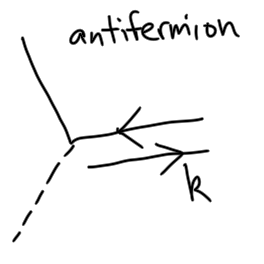
\includegraphics[scale=0.5]{antifermionket.png}  \end{figure}
	\subitem$ \wick[offset=1.5em]{\c {\bra{k,s}} \c {\hat{\psi}}} = v^s (k) = $ \begin{figure}[H]\centering 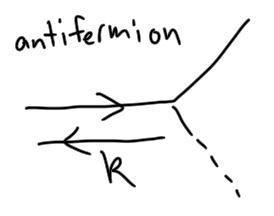
\includegraphics[scale=0.5]{antifermionbra.png}  \end{figure}
\item Conserve momentum at each vertex
\item Integrate over each loop momentum
\item Calculate the sign of the diagram
\item Divide by the symmetry factor
\end{enumerate}

\noindent Then the $n$-point Green's function is the sum of all connected and amputated Feynman diagrams with $n$ external legs subject to rules 1 through 7 above.

\noindent For example, a fermion scattering process looks like

\begin{figure}[H]\centering 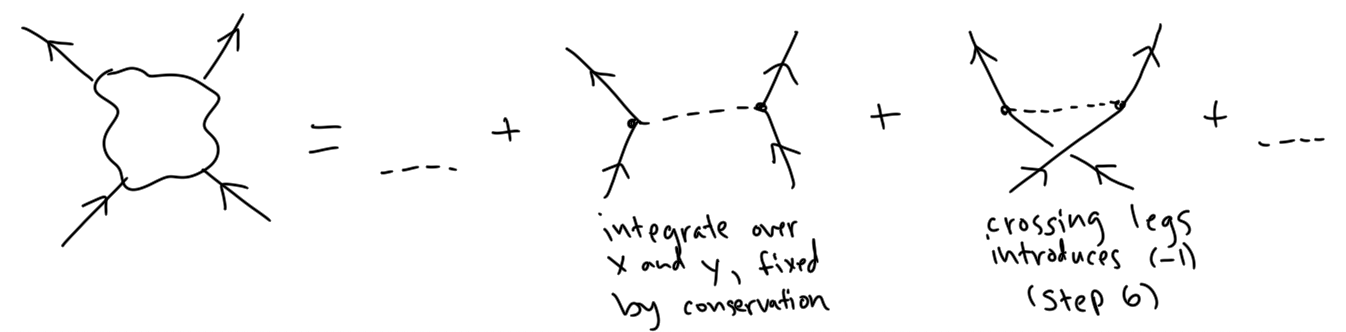
\includegraphics[scale=0.5]{fermionscattering.png}  \end{figure}